\documentclass[10pt,aspectratio=169]{beamer}

\usepackage[utf8]{inputenc}
\usepackage[T1]{fontenc}
\usepackage[provide=*,french]{babel}
\usepackage{lmodern}
\usepackage{booktabs}
\usepackage{array}
\usepackage{xcolor}
\usepackage{tikz}
\usetikzlibrary{positioning,arrows.meta,shapes.geometric}
\usepackage{amsmath}
\usepackage{hyperref}

\usetheme{Madrid}
\usecolortheme{seahorse}
\setbeamertemplate{navigation symbols}{}
\setbeamertemplate{caption}[numbered]
\setbeamerfont{footnote}{size=\tiny}

\definecolor{accent}{RGB}{30,90,160}
\setbeamercolor{title}{fg=accent}
\setbeamercolor{frametitle}{fg=accent}
\setbeamercolor{structure}{fg=accent}

\newcommand{\good}[1]{\textcolor{green!50!black}{#1}}
\newcommand{\bad}[1]{\textcolor{red!70!black}{#1}}
\newcommand{\code}[1]{\texttt{\small #1}}

% Freeze the slide counter for backup/appendix slides so they do not
% inflate the page count visible during the talk.
\newcommand{\backupbegin}{%
  \newcounter{finalframe}%
  \setcounter{finalframe}{\value{framenumber}}%
}
\newcommand{\backupend}{%
  \setcounter{framenumber}{\value{finalframe}}%
}

% Style for the Q/A boxes used in the appendix.
\newcommand{\qbox}[1]{\textit{\textcolor{accent}{Q : #1}}\par\smallskip}

\title[TTT auto-supervisé]{Test-Time Training auto-supervisé\\pour la classification d'images}
\subtitle{TER M1 VMI --- état d'avancement}
\author[Dolhov \& Diouf]{Maksym \textsc{Dolhov} \and Fallou \textsc{Diouf}}
\institute[U.~Paris]{Université Paris Cité --- M1 VMI}
\date{Mai 2026}

\begin{document}

% =====================================================================
\begin{frame}[plain]
  \titlepage
\end{frame}

% =====================================================================
\begin{frame}{Plan de l'exposé}
  \tableofcontents
\end{frame}

% =====================================================================
\section{Contexte et objectifs}

\begin{frame}{C'est quoi une \emph{distribution} ?}
  \begin{block}{Réponse intuitive}
    Une distribution, c'est la \alert{description de toutes les images que le modèle peut rencontrer} : lesquelles apparaissent, lesquelles sont fréquentes ou rares, et avec quelles étiquettes.
  \end{block}

  \begin{itemize}
    \item On la note $\mathcal{D}$ et on écrit $x \sim \mathcal{D}$ : « $x$ est tiré selon $\mathcal{D}$ ».
    \item On suppose les données d'entraînement \alert{i.i.d.} (indépendantes, même loi) :
    \[ (x_1, y_1), \dots, (x_n, y_n) \sim \mathcal{D}_{XY}. \]
    \item Concrètement, $\mathcal{D}$ pour CIFAR-10 répond à : \emph{quelles photos $32{\times}32$ peuvent apparaître, et avec quelles classes ?}
  \end{itemize}

  \vspace{0.4em}
  \begin{block}{Et un \emph{distribution shift} alors ?}
    Le modèle est entraîné sur $\mathcal{D}_{\text{train}}$, mais au test les données viennent d'une autre $\mathcal{D}_{\text{test}}$. \alert{Les règles du jeu changent entre l'entraînement et le test.}
  \end{block}

  \textbf{Dans notre cas} : CIFAR-10 (images propres) $\rightarrow$ CIFAR-10-C (mêmes objets mais bruit, flou, météo). Le \emph{contenu sémantique} reste --- un chien corrompu reste un chien --- mais l'apparence change.
\end{frame}

\begin{frame}{Contexte : robustesse à la dérive de distribution}
  \begin{columns}[T,onlytextwidth]
    \begin{column}{0.55\textwidth}
      \begin{itemize}
        \item Un classifieur entraîné sur un jeu propre perd souvent en performance dès que la distribution change : bruit, flou, météo, artefacts numériques.
        \item Problème récurrent en déploiement réel.
        \item Deux leviers étudiés dans le TER :
        \begin{itemize}
          \item \alert{Pré-entraînement auto-supervisé} (SimCLR) pour des représentations plus robustes ;
          \item \alert{Test-Time Training} (Sun et al., 2020) pour adapter le modèle au moment du test.
        \end{itemize}
      \end{itemize}
    \end{column}
    \begin{column}{0.42\textwidth}
      \centering
      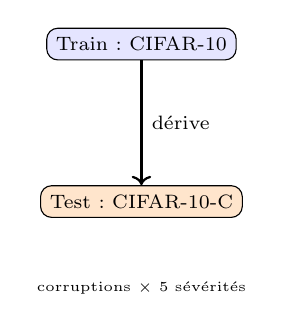
\begin{tikzpicture}[font=\scriptsize]
        \node[draw, rounded corners, fill=blue!10] (train) at (0,2) {Train : CIFAR-10};
        \node[draw, rounded corners, fill=orange!20] (test) at (0,0) {Test : CIFAR-10-C};
        \draw[->, thick] (train) -- node[right] {dérive} (test);
        \node[align=center, font=\tiny] at (0,-1.1) {corruptions $\times$ 5 sévérités};
      \end{tikzpicture}
    \end{column}
  \end{columns}
\end{frame}

\begin{frame}{Objectifs du TER}
  \begin{enumerate}
    \item Implémenter un pipeline complet de bout en bout :
    \begin{itemize}
      \item \textbf{SimCLR} pour le pré-entraînement auto-supervisé ;
      \item \textbf{ViT-Tiny} comme encodeur ;
      \item \textbf{CIFAR-10} pour l'entraînement, \textbf{CIFAR-10-C} pour l'évaluation sous dérive ;
      \item \textbf{TTT} pour l'adaptation au temps du test.
    \end{itemize}
    \item Mesurer l'effet de TTT (per-batch et per-image) sur l'accuracy.
    \item Identifier les régimes (corruption, sévérité) où TTT apporte un gain réel.
  \end{enumerate}

  \vspace{0.5em}
  \begin{block}{Aujourd'hui}
    Le pipeline tourne de bout en bout, un premier run overnight a été réalisé sur GPU L4 ; nous présentons les résultats préliminaires et discutons des prochaines étapes.
  \end{block}
\end{frame}

% =====================================================================
\section{Pipeline et méthode}

\begin{frame}{Vue d'ensemble du pipeline}
  \centering
  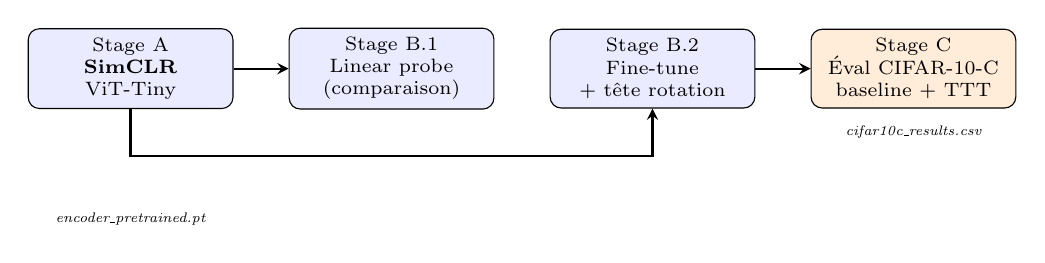
\begin{tikzpicture}[
      font=\scriptsize,
      node distance=0.7cm,
      box/.style={draw, rounded corners, minimum height=1cm, minimum width=2.6cm, align=center, fill=blue!8},
      arrow/.style={->, thick, >=stealth}
    ]
    \node[box]                          (a)  {Stage A\\\textbf{SimCLR}\\ViT-Tiny};
    \node[box, right=of a]              (b1) {Stage B.1\\Linear probe\\(comparaison)};
    \node[box, right=of b1]             (b2) {Stage B.2\\Fine-tune\\+ tête rotation};
    \node[box, right=of b2, fill=orange!15] (c) {Stage C\\Éval CIFAR-10-C\\baseline + TTT};

    \draw[arrow] (a) -- (b1);
    \draw[arrow] (a.south) |- ++(0,-0.6) -| (b2.south);
    \draw[arrow] (b2) -- (c);

    \node[below=1.2cm of a, font=\tiny\itshape, align=center] {encoder\_pretrained.pt};
    \node[below=0.1cm of c, font=\tiny\itshape, align=center] {cifar10c\_results.csv};
  \end{tikzpicture}

  \vspace{0.5em}
  \begin{itemize}\small
    \item Configuration centrale (\code{configs/default.yaml}), seeds fixes, AMP, AdamW + warmup/cosine.
    \item Préset \emph{smoke} (5~min) et \emph{default} (overnight L4).
  \end{itemize}
\end{frame}

\begin{frame}{Stage A --- SimCLR sur ViT-Tiny}
  \begin{columns}[T,onlytextwidth]
    \begin{column}{0.55\textwidth}
      \textbf{Pré-entraînement auto-supervisé}
      \begin{itemize}
        \item Deux vues augmentées par image (crop, color jitter, gray, blur).
        \item Perte contrastive \alert{NT-Xent} sur la projection $z = g(f(x))$.
        \item Encodeur : ViT-Tiny, patch $4{\times}4$, embed dim 192, drop\_path 0.1.
        \item Projection MLP $\to$ 128-d.
      \end{itemize}
      \textbf{Recipe}
      \begin{itemize}\small
        \item 200 époques, batch 1024, $\tau = 0{,}2$, lr $3\!\cdot\!10^{-3}$, warmup 10 ép., cosine, AMP.
      \end{itemize}
    \end{column}
    \begin{column}{0.42\textwidth}
      \centering
      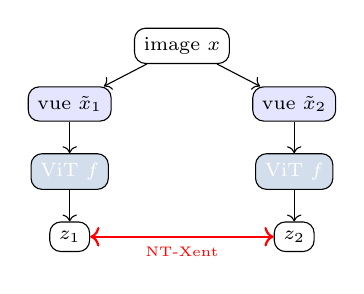
\begin{tikzpicture}[font=\scriptsize, node distance=0.4cm]
        \node[draw, rounded corners] (x) {image $x$};
        \node[draw, rounded corners, below left=of x, fill=blue!10] (v1) {vue $\tilde x_1$};
        \node[draw, rounded corners, below right=of x, fill=blue!10] (v2) {vue $\tilde x_2$};
        \node[draw, rounded corners, below=of v1, fill=accent!20, text=white] (f1) {ViT $f$};
        \node[draw, rounded corners, below=of v2, fill=accent!20, text=white] (f2) {ViT $f$};
        \node[draw, rounded corners, below=of f1] (z1) {$z_1$};
        \node[draw, rounded corners, below=of f2] (z2) {$z_2$};
        \draw[->] (x) -- (v1);
        \draw[->] (x) -- (v2);
        \draw[->] (v1) -- (f1); \draw[->] (f1) -- (z1);
        \draw[->] (v2) -- (f2); \draw[->] (f2) -- (z2);
        \draw[<->, thick, red] (z1) -- node[below, font=\tiny]{NT-Xent} (z2);
      \end{tikzpicture}
    \end{column}
  \end{columns}
\end{frame}

\begin{frame}{Stage B --- Fine-tuning et tête auxiliaire}
  \textbf{B.1 --- Linear probe} (comparaison)
  \begin{itemize}\small
    \item Encodeur gelé, classifieur linéaire, 30 époques. Sert de référence pour juger la qualité des représentations SimCLR.
  \end{itemize}

  \vspace{0.4em}
  \textbf{B.2 --- Fine-tune supervisé} (modèle principal)
  \begin{itemize}
    \item Encodeur dégelé, deux têtes en sortie :
    \begin{itemize}
      \item tête \textbf{classification} (10 classes, perte cross-entropy + label smoothing 0.1) ;
      \item tête \textbf{auxiliaire de rotation} (4 classes : $0^\circ, 90^\circ, 180^\circ, 270^\circ$).
    \end{itemize}
    \item Pertes combinées pendant l'entraînement.
    \item AdamW, lr $5\!\cdot\!10^{-4}$, weight decay 0.05, RandAugment, early stopping, AMP.
    \item La tête auxiliaire est conservée \alert{pour TTT au moment du test}.
  \end{itemize}
\end{frame}

\begin{frame}{Stage C --- Test-Time Training (Sun et al. 2020)}
  \begin{columns}[T,onlytextwidth]
    \begin{column}{0.55\textwidth}
      \textbf{Idée}
      \begin{itemize}\small
        \item Au test, on n'a pas les labels, mais on peut toujours résoudre la tâche auto-supervisée (rotation).
        \item Faire un pas de descente de gradient sur la perte rotation $\to$ adapter encodeur + tête rotation à la donnée de test.
        \item Puis prédire avec la tête de classification.
      \end{itemize}

      \textbf{Deux régimes implémentés}
      \begin{itemize}\small
        \item \alert{per-batch} : un pas par batch de test ;
        \item \alert{per-image} : un pas par image (128 copies tournées comme batch).
      \end{itemize}
    \end{column}
    \begin{column}{0.42\textwidth}
      \centering
      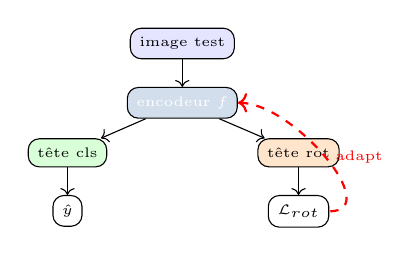
\begin{tikzpicture}[font=\tiny, node distance=0.35cm]
        \node[draw, rounded corners, fill=blue!10] (img) {image test};
        \node[draw, rounded corners, below=of img, fill=accent!20, text=white] (enc) {encodeur $f$};
        \node[draw, rounded corners, below left=of enc, fill=green!15] (cls) {tête cls};
        \node[draw, rounded corners, below right=of enc, fill=orange!20] (rot) {tête rot};
        \node[draw, rounded corners, below=of cls] (y) {$\hat y$};
        \node[draw, rounded corners, below=of rot] (lr) {$\mathcal L_{rot}$};
        \draw[->] (img)--(enc);
        \draw[->] (enc)--(cls); \draw[->] (cls)--(y);
        \draw[->] (enc)--(rot); \draw[->] (rot)--(lr);
        \draw[<-, red, thick, dashed] (enc.east) to[out=0,in=0] node[right]{adapt} (lr.east);
      \end{tikzpicture}
    \end{column}
  \end{columns}

  \vspace{0.3em}
  \begin{block}{Paramètres TTT}
    \small \code{lr=1e-3}, \code{steps=1}, \code{lambda\_rot=1.0}, \code{adapt\_scope=encoder\_plus\_head}, snapshot/reset entre chaque (corruption, sévérité).
  \end{block}
\end{frame}

\begin{frame}{Architecture du dépôt}
  \centering
  \small
  \begin{tabular}{ll}
    \toprule
    Module & Rôle \\
    \midrule
    \code{src/core/}        & pipeline orchestration, config dataclass \\
    \code{src/data/}        & datasets CIFAR-10 / CIFAR-10-C, 3 transforms \\
    \code{src/models/}      & ViT-Tiny backbone, SimCLR, classifier+rot head \\
    \code{src/training/}    & SimCLR / linear probe / fine-tune trainers \\
    \code{src/ttt/}         & adapter Sun~2020 (rotation), \code{rotate\_batch} \\
    \code{src/evaluation/}  & boucle CIFAR-10-C avec/sans TTT, métriques \\
    \code{src/utils/}       & logger, checkpoints, seed \\
    \code{configs/}         & \code{smoke.yaml}, \code{default.yaml} \\
    \code{notebooks/}       & \code{colab.ipynb} (run de bout en bout) \\
    \bottomrule
  \end{tabular}

  \vspace{0.6em}
  \begin{itemize}\footnotesize
    \item Code modulaire, $\sim$2\,500 lignes Python, configurable par YAML.
    \item Une seule entrée : \code{python main.py --config configs/default.yaml}.
  \end{itemize}
\end{frame}

% =====================================================================
\section{Résultats préliminaires}

\begin{frame}{Setup d'évaluation}
  \begin{itemize}
    \item Run overnight unique sur GPU L4 (seed 42).
    \item \textbf{Stage C} : 14 corruptions\footnote{14 sur les 15 corruptions standard de Hendrycks~2019 --- détail en \textbf{Annexe A}.} $\times$ 5 sévérités sur CIFAR-10-C, soit 70 cellules.
    \item Pour chaque cellule on calcule :
    \begin{itemize}
      \item \textbf{baseline} (10\,000 images, sans adaptation),
      \item \textbf{per-batch TTT} (10\,000 images, un pas par batch),
      \item \textbf{per-image TTT} (sous-échantillon stratifié de 1\,000 images, un pas par image).
    \end{itemize}
    \item Per-image limité à 1\,000 images : 128 copies tournées par image $\Rightarrow$ coût $\sim$20\,h L4 sur les 70k.
    \item Reset des poids entre chaque (corruption, sévérité) pour éviter la fuite d'adaptation.
  \end{itemize}
\end{frame}

\begin{frame}{Accuracy sur données propres (CIFAR-10 clean)}
  \centering
  \begin{tabular}{lc}
    \toprule
    \textbf{Configuration} & \textbf{Top-1} \\
    \midrule
    Stage B.2 fine-tune (val, époque 30, best) & \textbf{0,9008} \\
    Stage C clean --- baseline (sans TTT)      & 0,8959 \\
    Stage C clean --- per-batch TTT            & 0,8960 \;($\Delta\!+\!0{,}0001$) \\
    Stage C clean --- per-image TTT (sous-éch. 1k) & 0,8980 \\
    \bottomrule
  \end{tabular}

  \vspace{1em}
  \begin{itemize}
    \item Aucune dégradation sur les données propres : la tête auxiliaire ne casse pas le classifieur quand on l'adapte au test.
    \item Bon sanity check avant de regarder CIFAR-10-C.
  \end{itemize}
\end{frame}

\begin{frame}{CIFAR-10-C --- accuracy moyenne par sévérité}
  \centering
  \small
  \begin{tabular}{r|ccc|cc}
    \toprule
    Sévérité & baseline & per-batch & per-image (1k) & $\Delta$ batch & $\Delta$ image* \\
    \midrule
    1 & 0,8673 & 0,8679 & 0,8666 & \good{+0,0007} & \bad{$-$0,0006} \\
    2 & 0,8392 & 0,8409 & 0,8395 & \good{+0,0017} & +0,0003 \\
    3 & 0,8033 & 0,8059 & 0,8033 & \good{+0,0025} & ~0,0000 \\
    4 & 0,7516 & 0,7575 & 0,7534 & \good{+0,0059} & \good{+0,0018} \\
    5 & 0,6803 & 0,6890 & 0,6830 & \good{+0,0087} & \good{+0,0027} \\
    \midrule
    \textbf{moyenne} & \textbf{0,7883} & \textbf{0,7922} & \textbf{0,7892} & \good{\textbf{+0,0039}} & \textbf{+0,0009} \\
    \bottomrule
  \end{tabular}

  \vspace{0.6em}
  \begin{itemize}\footnotesize
    \item Per-batch : gain qui croît avec la sévérité (+0,07~pp à sév.~1 $\to$ +0,87~pp à sév.~5).
    \item *$\Delta$ image vs baseline 10k. Sur le sous-ensemble apparié 1k (apples-to-apples), per-image donne $\Delta$ moyen de \bad{$-0{,}0048$}.
  \end{itemize}
\end{frame}

\begin{frame}{Wins / losses par cellule (70 cellules, sévérité $\geq$ 1)}
  \centering
  \begin{tabular}{lccc}
    \toprule
    Mode & wins & losses & ties \\
    \midrule
    per-batch (vs baseline 10k)            & \good{\textbf{61}} & 6   & 3 \\
    per-image (vs baseline appariée 1k)    & 16   & \bad{\textbf{46}} & 8 \\
    \bottomrule
  \end{tabular}

  \vspace{1em}
  \begin{itemize}
    \item \textbf{Per-batch :} 61/70 cellules améliorées, 6 régressions mineures, signature attendue de Sun~2020.
    \item \textbf{Per-image :} sur sous-ensemble apparié, 46/70 cellules régressent. Le mode dégrade nettement dans notre setup.
  \end{itemize}
\end{frame}

\begin{frame}{Top des gains per-batch (toutes sévérités confondues)}
  \centering
  \begin{tabular}{lcccc}
    \toprule
    Corruption & sévérité & baseline & per-batch & $\Delta$ \\
    \midrule
    fog            & 5 & 0,5367 & 0,5586 & \good{\textbf{+0,0219}} \\
    pixelate       & 5 & 0,7378 & 0,7530 & \good{+0,0152} \\
    impulse\_noise & 5 & 0,3959 & 0,4109 & \good{+0,0150} \\
    pixelate       & 4 & 0,7634 & 0,7772 & \good{+0,0138} \\
    impulse\_noise & 4 & 0,5547 & 0,5675 & \good{+0,0128} \\
    gaussian\_noise & 4 & 0,5556 & 0,5679 & \good{+0,0123} \\
    \bottomrule
  \end{tabular}

  \vspace{0.7em}
  \begin{itemize}
    \item Les gains se concentrent sur les corruptions \emph{lourdes} (sév. 4--5) : brouillard, pixelisation forte, bruits.
    \item Sévérité 4 ressort souvent plus que la 5 : à sév. 5 le baseline est déjà très dégradé (gaussian\_noise s5 = $49{,}6\,\%$), il reste moins de signal à récupérer.
    \item Régimes où la tâche prétexte de rotation a le plus à donner.
  \end{itemize}
\end{frame}

\begin{frame}{Ablations TTT --- effet de \code{steps} et \code{lr}}
  Trois configurations exécutées de bout en bout sur les 70 cellules de CIFAR-10-C :

  \vspace{0.4em}
  \centering
  \small
  \begin{tabular}{lcc|cc}
    \toprule
    Configuration & \multicolumn{2}{c|}{per-batch ($\Delta$ moyen)} & \multicolumn{2}{c}{per-image ($\Delta$ moyen, 1k matched)} \\
                  & toutes sév. & sév. 5 only & toutes sév. & sév. 5 only \\
    \midrule
    \textbf{Default} (\code{steps=1, lr=1e-3}) & \good{+0,39~pp} & \good{+0,87~pp} & \bad{$-$0,48~pp} & \bad{$-$1,24~pp} \\
    \textbf{steps=5} (\code{lr=1e-3})          & \good{\textbf{+1,50~pp}} & \good{\textbf{+3,21~pp}} & \bad{\textbf{$-$1,68~pp}} & \bad{\textbf{$-$3,97~pp}} \\
    \textbf{lr=1e-4} (\code{steps=1})          & +0,04~pp        & +0,10~pp        & $-$0,05~pp       & $-$0,11~pp \\
    \bottomrule
  \end{tabular}

  \vspace{0.6em}
  \begin{itemize}\footnotesize
    \item \alert{\code{steps=5} amplifie les deux effets en miroir} : per-batch passe à 67/70 wins (max +6,78~pp à fog s5) ; per-image chute à 9/57 wins (min $-9{,}20$~pp à impulse\_noise s5).
    \item \code{lr=1e-4} étouffe le gradient d'adaptation $\Rightarrow$ TTT devient inopérant (signaux à $\sim 0$).
    \item Diagnostic : \emph{plus on adapte, plus le per-image se dégrade} $\Rightarrow$ confirme l'hypothèse de sur-adaptation sur ViT/LN.
  \end{itemize}
\end{frame}

\begin{frame}{Résumé quantitatif des runs}
  \centering
  \small
  \begin{tabular}{lcccc}
    \toprule
    Run & per-batch & per-image (1k) & wins/losses (per-batch) & wins/losses (per-image) \\
    \midrule
    Default            & \good{+0,39~pp} & \bad{$-$0,48~pp} & 61 / 6 / 3   & 16 / 46 / 8 \\
    steps=5            & \good{+1,50~pp} & \bad{$-$1,68~pp} & \good{67 / 2 / 1} & \bad{9 / 57 / 4} \\
    lr=1e-4            & +0,04~pp        & $-$0,05~pp       & 45 / 12 / 13 & 10 / 25 / 35 \\
    \bottomrule
  \end{tabular}
  \par\vspace{0.2em}\scriptsize{\emph{Format : wins / losses / ties sur 70 cellules (sévérité $\geq 1$).}}

  \vspace{0.7em}
  \begin{block}{Lecture en une phrase}
    Seul \alert{per-batch avec adaptation \emph{plus agressive} (\code{steps=5})} produit des gains francs et fiables (+1,5~pp moyen, +3,2~pp à sévérité~5, 67/70 cellules améliorées). \\ Per-image dégrade systématiquement, et l'effet s'aggrave quand on adapte plus.
  \end{block}
\end{frame}

% =====================================================================
\section{Interprétation et prochaines étapes}

\begin{frame}{Interprétation des résultats}
  \begin{enumerate}
    \item \textbf{Per-batch TTT fonctionne} comme attendu :
    \begin{itemize}\small
      \item gain modeste mais cohérent qui croît avec la sévérité,
      \item 61/70 cellules améliorées, aucun effet négatif sur les données propres,
      \item compatible avec la signature publiée par Sun et al. 2020.
    \end{itemize}

    \item \textbf{Per-image TTT dégrade} dans notre configuration ViT/LayerNorm :
    \begin{itemize}\small
      \item ViT utilise \alert{LayerNorm} : pas de régularisation par statistiques de batch, contrairement aux backbones BN sur lesquels TTT a été conçu ;
      \item 128 copies tournées d'une seule image $\Rightarrow$ signal mince ;
      \item le scope \emph{encoder + head} peut être trop large pour un seul pas par image $\Rightarrow$ dérive de l'encodeur.
    \end{itemize}

    \item \textbf{L'ablation \code{steps=5} confirme l'hypothèse de sur-adaptation} : per-batch s'améliore encore (+1,5~pp moyen, 67/70 wins), per-image s'effondre davantage ($-1{,}68$~pp moyen, jusqu'à $-9{,}2$~pp). Adapter \emph{plus} aide en mode batch et casse en mode image.

    \item \textbf{Gains concentrés sur les corruptions lourdes} : c'est là que le pretexte de rotation a le plus à apporter.
  \end{enumerate}
\end{frame}

\begin{frame}{Limitations actuelles}
  \begin{itemize}
    \item Une seule seed $\Rightarrow$ pas de barres de variance.
    \item Per-image évalué sur 1\,000 images seulement (contrainte de coût).
    \item Ablations partielles : seulement \code{steps} (1, 5) et \code{lr} (1e-3, 1e-4) explorés ; \code{adapt\_scope}, \code{lambda\_rot} et \code{rotation\_mode} pas encore balayés.
    \item Comparaison à TTT-BN (style Sun original avec ResNet) absente $\Rightarrow$ on ne peut pas isoler l'effet ViT/LN du reste.
    \item Pas encore de comparaison avec des baselines hors TTT (ex.~Tent, BN-stats adaptation).
  \end{itemize}
\end{frame}

\begin{frame}{Prochaines étapes envisagées}
  \begin{itemize}
    \item \textbf{Compléter les ablations} (déjà : steps=5, lr=1e-4) :
    \begin{itemize}\small
      \item lr $\in \{10^{-4}, 10^{-3}, 10^{-2}\}$, steps $\in \{1, 5, 10\}$ ;
      \item scope d'adaptation : \emph{head only}, \emph{LN only}, \emph{encoder + head}.
    \end{itemize}
    \item \textbf{Variance} : 3 seeds sur le pipeline complet pour des barres d'erreur.
    \item \textbf{Comparatif} : ResNet18 BN + TTT comme référence (vérifier l'hypothèse LN vs BN).
    \item \textbf{Aller plus loin} (selon le temps) : ActMAD, Tent, comparaison avec TTT-MAE.
    \item \textbf{Rédaction} du rapport final + figures consolidées (par corruption, courbes severité).
  \end{itemize}
\end{frame}

% =====================================================================
\section{Conclusion}

\begin{frame}{Conclusion}
  \begin{itemize}
    \item Pipeline complet \alert{opérationnel} : SimCLR (ViT-Tiny) $\to$ fine-tune avec tête rotation $\to$ évaluation CIFAR-10-C avec et sans TTT.
    \item Premier run overnight reproduit la signature attendue de TTT en mode \textbf{per-batch} (+0,4~pp en moyenne, croissant avec la sévérité).
    \item Mode \textbf{per-image} dégrade dans notre setup ViT/LN $\Rightarrow$ piste d'investigation principale.
    \item Code public et reproductible :
    \begin{center}\small
      \href{https://github.com/3v3r51nc3/SelfSupervised-TTT-ImageClassification}{\code{github.com/3v3r51nc3/SelfSupervised-TTT-ImageClassification}}
    \end{center}
  \end{itemize}

  \vspace{0.6em}
  \begin{block}{Objectifs du rendez-vous}
    \begin{enumerate}\small
      \item Vérifier que l'implémentation correspond aux attentes du sujet.
      \item Discuter des prochaines ablations à prioriser.
      \item Recueillir vos retours sur le mode per-image.
    \end{enumerate}
  \end{block}
\end{frame}

% =====================================================================
\begin{frame}{Questions pour vous --- 1/2 : alignement et ablations}
  \textbf{1. Alignement avec le sujet du TER}
  \begin{itemize}\small
    \item ViT-Tiny (patch~$4{\times}4$, embed~192) --- taille adaptée, ou faut-il viser ViT-Small ?
    \item Architecture en Y avec tête rotation entraînée \emph{conjointement} en Stage B.2 --- bien ce que vous attendiez, ou tête détachée préférable ?
    \item Choix de Sun~2020 (rotation) plutôt que TTT++ (NT-Xent) au moment du test --- conforme au sujet, ou TTT++ attendu en plus ?
    \item Scope d'adaptation \code{encoder + tête rotation} (classifieur gelé) --- bon choix, ou restreindre aux paramètres LN seulement ?
    \item Évaluation per-image sur 1\,k images au lieu des 10\,k --- acceptable pour le rapport final ?
  \end{itemize}

  \vspace{0.4em}
  \textbf{2. Ablations à prioriser}
  \begin{itemize}\small
    \item 3~seeds pour variance --- obligatoire, ou 1~seed acceptable au stade actuel ?
    \item ResNet18+BN comme expérience-contrôle pour isoler l'effet LN --- indispensable, ou nice-to-have ?
    \item Ablation \code{adapt\_scope} (head\_only / LN\_only / encoder+head) --- prioritaire ?
    \item Ajout de \code{zoom\_blur} pour passer à 15/15 corruptions --- attendu pour le rapport ?
    \item Comparaison à au moins une baseline non-Sun (Tent ou ActMAD) --- demandée ?
  \end{itemize}
\end{frame}

\begin{frame}{Questions pour vous --- 2/2 : ressources et livrables}
  \textbf{3. Ressources de calcul}
  \begin{itemize}\small
    \item Notre crédit Colab Pro est épuisé. Possibilités côté laboratoire ou université :
    \begin{itemize}\footnotesize
      \item GPU partagés du laboratoire LIPADE / accès SSH ?
      \item Budget Google Cloud / AWS éducation ?
    \end{itemize}
    \item Estimation de notre besoin restant : $\sim$30--40~h L4 équivalent (3~seeds $\times$ 2~configs + ResNet contrôle + ablations \code{adapt\_scope}).
  \end{itemize}

  \vspace{0.4em}
  \textbf{4. Livrables et organisation}
  \begin{itemize}\small
    \item Format et longueur attendus pour le rapport final ?
    \item Date approximative de la soutenance ?
  \end{itemize}
\end{frame}

\begin{frame}[allowframebreaks]{Références}
  \footnotesize
  \begin{thebibliography}{99}
    \setbeamertemplate{bibliography item}[text]

    \bibitem{Sun2020}
      Y.~Sun, X.~Wang, Z.~Liu, J.~Miller, A.~Efros, M.~Hardt.
      \newblock \emph{Test-time training with self-supervision for generalization under distribution shifts}.
      \newblock ICML, 2020. \href{https://arxiv.org/abs/1909.13231}{arXiv:1909.13231}.

    \bibitem{Liu2021}
      Y.~Liu, P.~Kothari, B.~Van~Delft, B.~Bellot-Gurlet, T.~Mordan, A.~Alahi.
      \newblock \emph{TTT++: When does self-supervised test-time training fail or thrive?}
      \newblock NeurIPS, 2021.

    \bibitem{Han2025}
      J.~Han, J.~Park, D.~Han, W.~Hwang.
      \newblock \emph{When Test-Time Adaptation Meets Self-Supervised Models}.
      \newblock \href{https://arxiv.org/abs/2506.23529}{arXiv:2506.23529}, 2025.

    \bibitem{Mirza2023}
      M.~J.~Mirza, P.~Jané~Soneira, W.~Lin, M.~Kozinski, H.~Possegger, H.~Bischof.
      \newblock \emph{ActMAD: Activation matching to align distributions for test-time training}.
      \newblock CVPR, 2023.

    \bibitem{Chen2020}
      T.~Chen, S.~Kornblith, M.~Norouzi, G.~Hinton.
      \newblock \emph{A Simple Framework for Contrastive Learning of Visual Representations} (SimCLR).
      \newblock ICML, 2020. \href{https://arxiv.org/abs/2002.05709}{arXiv:2002.05709}.

    \bibitem{Dosovitskiy2021}
      A.~Dosovitskiy et~al.
      \newblock \emph{An Image is Worth 16x16 Words: Transformers for Image Recognition at Scale} (ViT).
      \newblock ICLR, 2021. \href{https://arxiv.org/abs/2010.11929}{arXiv:2010.11929}.

    \bibitem{Hendrycks2019}
      D.~Hendrycks, T.~Dietterich.
      \newblock \emph{Benchmarking Neural Network Robustness to Common Corruptions and Perturbations} (CIFAR-10-C).
      \newblock ICLR, 2019. \href{https://arxiv.org/abs/1903.12261}{arXiv:1903.12261}.

    \bibitem{Gidaris2018}
      S.~Gidaris, P.~Singh, N.~Komodakis.
      \newblock \emph{Unsupervised Representation Learning by Predicting Image Rotations}.
      \newblock ICLR, 2018. \href{https://arxiv.org/abs/1803.07728}{arXiv:1803.07728}.

    \bibitem{Krizhevsky2009}
      A.~Krizhevsky.
      \newblock \emph{Learning Multiple Layers of Features from Tiny Images} (CIFAR-10/100).
      \newblock Tech.~report, U.~Toronto, 2009.

  \end{thebibliography}
\end{frame}

\begin{frame}[plain]
  \begin{center}
    \vspace{1.5cm}
    {\Huge\color{accent}\textbf{Merci de votre attention}}\\[1.5em]
    {\Large Questions ?}\\[2em]
    {\small Maksym \textsc{Dolhov} \quad\textbullet\quad Fallou \textsc{Diouf}}\\
    {\footnotesize TER M1 VMI --- Université Paris Cité --- Mai 2026}
  \end{center}
\end{frame}

% =====================================================================
% =============== ANNEXES / BACKUP / Q\&A PRÉPARÉ ======================
% =====================================================================
\backupbegin

\appendix
\section*{Annexes}

\begin{frame}[plain]
  \begin{center}
    \vspace{2cm}
    {\Huge\color{accent}\textbf{Annexes}}\\[1em]
    {\large Slides de réserve --- Q\&A préparé}
  \end{center}
\end{frame}

% --- A1 : 14/15 corruptions ------------------------------------------
\begin{frame}{Annexe A --- Pourquoi 14 corruptions et non 15 ?}
  \qbox{\guillemotleft\,Le benchmark CIFAR-10-C standard (Hendrycks \& Dietterich, 2019) en compte 15. Pourquoi 14 ?\,\guillemotright{}}

  \begin{itemize}
    \item Notre liste codée en dur (\code{src/data/dataset.py}) couvre 14 des 15 corruptions standard ; il manque \alert{\code{zoom\_blur}}.
    \item Repéré après le run overnight en relisant Hendrycks --- \emph{oubli} de notre part dans la liste, pas un choix méthodologique.
    \item Les 4 \textbf{familles} du benchmark (noise, blur, weather, digital) restent toutes représentées :
    \begin{itemize}\small
      \item noise : gaussian, shot, impulse \quad blur : defocus, glass, motion
      \item weather : snow, frost, fog, brightness \quad digital : contrast, elastic, pixelate, jpeg
    \end{itemize}
    \item La lecture qualitative (\emph{per-batch fonctionne, per-image dégrade, gains croissants avec sévérité}) ne dépend pas d'\code{zoom\_blur}.
    \item \textbf{Action} : ajout d'\code{zoom\_blur} et rerun de Stage C avant le rapport final ($\sim$30~min de marginal sur L4).
  \end{itemize}
\end{frame}

% --- A2 : Single seed -------------------------------------------------
\begin{frame}{Annexe B --- Seed unique, comment quantifier le bruit ?}
  \qbox{\guillemotleft\,Comment savez-vous que le +0,4~pp de per-batch n'est pas du bruit de seed ?\,\guillemotright{}}

  \begin{itemize}
    \item \textbf{Honnêtement : nous ne le savons pas encore.} Le run présenté est sur une seule seed (42).
    \item Indices indirects qui suggèrent que ce n'est pas du bruit pur :
    \begin{itemize}\small
      \item monotonie sur la sévérité ($+0{,}07 \to +0{,}87$~pp), peu probable par chance ;
      \item 61/70 cellules améliorées (binomial $p \!<\! 10^{-12}$ contre 50/50) ;
      \item zéro régression sur \code{clean} --- adaptation contrôlée.
    \end{itemize}
    \item Plan : 3 seeds (42, 1337, 2024) avec mêmes hyperparamètres pour barres d'erreur ; coût $\sim$6~h L4.
    \item Pour la per-image dégradation ($\Delta = -0{,}48$~pp sur 1k), le signe est cohérent à travers toutes les sévérités $\geq$ 1 ; même argument de monotonie tient.
  \end{itemize}
\end{frame}

% --- A3 : ViT/LN vs ResNet/BN ----------------------------------------
\begin{frame}{Annexe C --- ViT/LN vs ResNet/BN : choix défendable ?}
  \qbox{\guillemotleft\,Sun~2020 utilise ResNet-26 + BatchNorm. Vous changez backbone ET norme : comment isoler les effets ?\,\guillemotright{}}

  \begin{itemize}
    \item Choix de ViT-Tiny motivé par :
    \begin{itemize}\small
      \item le sujet du TER demande explicitement \emph{ViT comme encodeur} (cf. consigne TER2.pdf) ;
      \item compatibilité directe avec SimCLR (representations \code{[CLS]}) sans modification d'architecture ;
      \item coût gérable sur L4 vs ViT-S/B.
    \end{itemize}
    \item Conséquence reconnue : LayerNorm n'a pas de statistiques de batch à recalibrer $\Rightarrow$ TTT par batch \emph{ne peut pas} bénéficier du même mécanisme que le TTT-BN original.
    \item Notre +0,4~pp est donc \alert{purement par adaptation des poids via la perte rotation}, pas via une renormalisation BN.
    \item \textbf{Ablation prévue} : refaire l'expérience avec ResNet-18 + BN dans le même pipeline pour isoler la contribution de la norme.
  \end{itemize}
\end{frame}

% --- A4 : Per-image hypothesis unfalsified ---------------------------
\begin{frame}{Annexe D --- L'hypothèse \guillemotleft\,per-image dégrade à cause de LN\,\guillemotright{} est-elle testée ?}
  \qbox{\guillemotleft\,Vous avancez 3 hypothèses pour la régression per-image. Laquelle est démontrée ?\,\guillemotright{}}

  \begin{itemize}
    \item \textbf{Aucune n'est démontrée}, ce sont des hypothèses ordonnées par plausibilité --- nous l'assumons explicitement.
    \item Plan d'ablation pour \emph{falsifier} chacune :
    \begin{itemize}\small
      \item \alert{LN vs BN} : ResNet-18 + BN identique. Si per-image gagne sur ResNet $\Rightarrow$ hypothèse 1 confirmée.
      \item \alert{Signal mince (128 copies)} : varier \code{per\_image\_aug\_k} $\in \{16, 64, 128, 256\}$. Si la dégradation s'atténue avec $k$ croissant $\Rightarrow$ hypothèse 2.
      \item \alert{Scope trop large} : \code{adapt\_scope $\in$ \{head\_only, ln\_only, encoder+head\}}. Si \emph{ln\_only} ou \emph{head\_only} récupère, hypothèse 3.
    \end{itemize}
    \item Runs \code{ablation-lr-1e-4} et \code{ablation-steps-5} déjà lancés ; structure prête pour les autres axes.
  \end{itemize}
\end{frame}

% --- A5 : Hyperparameter selection / leakage --------------------------
\begin{frame}{Annexe E --- Tuning et risque de fuite de test}
  \qbox{\guillemotleft\,Sur quoi avez-vous tuné \code{lr}, \code{steps}, \code{lambda\_rot}, \code{adapt\_scope} ? Pas sur CIFAR-10-C j'espère ?\,\guillemotright{}}

  \begin{itemize}
    \item Hyperparamètres TTT \alert{n'ont pas été tunés} sur CIFAR-10-C : valeurs reprises directement de Sun~2020 (\code{lr=1e-3}, \code{steps=1}, \code{lambda\_rot=1.0}).
    \item Hyperparamètres SimCLR / fine-tune choisis sur la \textbf{val split} de CIFAR-10 (10\% du train), CIFAR-10-C jamais vu pendant le tuning.
    \item Les ablations à venir (lr, steps, scope) seront menées sur le \alert{validation set des 4 corruptions \guillemotleft\,extra\,\guillemotright{}} de Hendrycks (\code{speckle\_noise, gaussian\_blur, spatter, saturate}), précisément le rôle pour lequel elles sont conçues.
    \item Le rapport final reportera les nombres finaux uniquement sur les 15 corruptions \guillemotleft\,test\,\guillemotright{}, sans tuning post-hoc.
  \end{itemize}
\end{frame}

% --- A6 : No comparison baselines (Tent, BN-stats, etc.) -------------
\begin{frame}{Annexe F --- Pourquoi pas de comparaison avec Tent / SAR / BN-stats ?}
  \qbox{\guillemotleft\,Sun~2020 c'est 2020. Pourquoi pas Tent (2021), EATA (2022), SAR (2023) ?\,\guillemotright{}}

  \begin{itemize}
    \item Le sujet du TER cite explicitement \textbf{Sun~2020} [1] et \textbf{TTT++ (Liu~2021)} [2] comme références principales --- nous avons commencé par [1] qui est la formulation canonique du TTT auto-supervisé.
    \item Comparer à Tent / SAR sortirait du cadre direct du sujet et nécessiterait :
    \begin{itemize}\small
      \item d'implémenter une seconde tête / mécanisme d'adaptation ;
      \item de standardiser les budgets de calcul (Tent fait 1 backward sur entropy seulement, Sun fait un pas via rotation, ce n'est pas directement comparable).
    \end{itemize}
    \item Extension naturelle si le temps le permet : ajouter Tent ou TTT++ comme seconde baseline pour situer notre résultat dans le paysage TTT.
    \item Tent / EATA / SAR mentionnés en related work du rapport.
  \end{itemize}
\end{frame}

% --- A7 : Cost / latency of TTT ---------------------------------------
\begin{frame}{Annexe G --- Coût computationnel de TTT}
  \qbox{\guillemotleft\,Vous gagnez 0,4~pp avec per-batch et 4--8~pp à sévérité 5. Combien ça coûte en temps d'inférence ?\,\guillemotright{}}

  \centering
  \begin{tabular}{lcc}
    \toprule
    Mode & gain moyen & sur-coût d'inférence \\
    \midrule
    baseline           & --- & 1$\times$ (forward seul) \\
    per-batch TTT      & +0,4~pp ($\sim$+0,9~pp à sév.~5) & $\sim$2$\times$ (1 fwd + 1 bwd) \\
    per-image TTT      & $-0{,}5$~pp & $\sim$130$\times$ (128 copies + bwd) \\
    \bottomrule
  \end{tabular}

  \vspace{0.7em}
  \begin{itemize}\small
    \item Per-batch double l'inférence pour un gain modeste --- compromis raisonnable en déploiement où la robustesse compte.
    \item Per-image \alert{n'est jamais rentable} dans notre setup : plus lent ET pire en accuracy.
    \item Cost-accuracy curve à inclure dans le rapport.
  \end{itemize}
\end{frame}

% --- A8 : Reset semantics --------------------------------------------
\begin{frame}{Annexe H --- Reset entre (corruption, sévérité) : choix réaliste ?}
  \qbox{\guillemotleft\,En vrai déploiement on a un \emph{stream} continu, pas 70 cases isolées. Pourquoi reset entre chaque ?\,\guillemotright{}}

  \begin{itemize}
    \item Reset est un choix \alert{méthodologique} pour mesurer \emph{l'effet de TTT en isolation}, conformément au protocole de Sun~2020 :
    \begin{itemize}\small
      \item sans reset, l'adaptation cumule et masque la contribution propre à chaque type de dérive ;
      \item avec reset, on lit chaque (corruption, sévérité) comme un test indépendant.
    \end{itemize}
    \item Pas réaliste pour un déploiement, oui --- mais c'est l'angle du papier de référence.
    \item Le scénario \emph{continual TTT} (sans reset, dérive qui change dans le temps) est une ligne de recherche distincte (Wang et al. 2022, EATA) qui pourrait constituer une extension du TER.
    \item Notre code expose le reset comme un toggle $\Rightarrow$ trivial à désactiver pour une expérience continual.
  \end{itemize}
\end{frame}

% --- A9 : Why SimCLR + rotation pretext, not MAE / DINO --------------
\begin{frame}{Annexe I --- Pourquoi SimCLR et rotation, pas MAE / DINO ?}
  \qbox{\guillemotleft\,2020 c'est ancien. SimCLR + rotation, pas un peu daté pour un ViT ?\,\guillemotright{}}

  \begin{itemize}
    \item Choix dicté par le sujet TER (SimCLR pour pré-entraînement, Sun~2020 pour TTT).
    \item Justification scientifique néanmoins :
    \begin{itemize}\small
      \item SimCLR reste un baseline contrastif solide, bien compris, peu coûteux ($\sim$2~h L4 vs $\sim$10~h pour MAE comparable) ;
      \item Rotation est la tâche prétexte la plus simple à coupler avec une tête auxiliaire pendant le fine-tune ;
      \item Plus important : on étudie \emph{l'effet de TTT}, pas l'optimum de SSL. Tant que la représentation est compétente, la conclusion sur TTT reste valide.
    \end{itemize}
    \item Extension possible : remplacer SimCLR par DINO ou MAE et regarder si le signal TTT change qualitativement.
  \end{itemize}
\end{frame}

% --- A10 : SimCLR vs rotation : où est utilisé SimCLR ? ---------------
\begin{frame}{Annexe J --- \guillemotleft\,Où est SimCLR exactement ?\,\guillemotright{}}
  \qbox{\guillemotleft\,Vous deviez utiliser SimCLR. Or au moment du test vous adaptez via une perte rotation. SimCLR est-il vraiment utilisé ?\,\guillemotright{}}

  \textbf{Oui, SimCLR est central dans le pipeline --- mais à une étape précise :}

  \vspace{0.4em}
  \centering
  \small
  \begin{tabular}{lll}
    \toprule
    Étape & Tâche prétexte & Loss \\
    \midrule
    Stage A --- pré-entraînement     & \alert{SimCLR} (2 vues augmentées) & \alert{NT-Xent}, 200 époques \\
    Stage B.2 --- fine-tune          & rotation auxiliaire (4 angles)     & CE classif + CE rotation \\
    Stage C --- TTT (Sun~2020 [1])   & rotation auxiliaire                 & CE rotation seule \\
    \bottomrule
  \end{tabular}

  \vspace{0.6em}
  \begin{itemize}\small
    \item Les représentations de l'encodeur ViT sont \alert{intégralement issues de SimCLR} (Stage~A) --- sans cette pré-tâche, pas de modèle.
    \item Au moment du \emph{test}, le sujet [1, Sun~2020] spécifie la rotation comme tâche prétexte d'adaptation $\Rightarrow$ c'est ce que nous utilisons.
    \item La projection SimCLR est jetée après Stage~A (pratique standard du papier original).
  \end{itemize}
\end{frame}

% --- A11 : Variante TTT++ (NT-Xent dans le TTT) -----------------------
\begin{frame}{Annexe K --- Et si vous vouliez du contrastive \emph{aussi} pendant le TTT ?}
  \qbox{\guillemotleft\,Pourquoi ne pas utiliser NT-Xent au moment du test, comme TTT++ (Liu~2021) ?\,\guillemotright{}}

  \begin{itemize}
    \item C'est la variante de la deuxième référence du sujet : \textbf{[2] Liu et al., TTT++ (NeurIPS~2021)}. Conceptuellement légitime, complémentaire de Sun~2020 [1].
    \item \textbf{Notre choix actuel} : commencer par [1] Sun~2020 (rotation), formulation canonique et plus simple à implémenter de bout en bout.
    \item \textbf{Extension TTT++ peu coûteuse à ajouter} : notre pipeline est structuré pour, il suffirait de :
    \begin{itemize}\small
      \item conserver la tête de projection SimCLR au-delà de Stage~A (au lieu de la jeter),
      \item à l'inférence : générer 2 vues augmentées par image, calculer NT-Xent, faire un pas SGD,
      \item remplacer \code{\_rotation\_step()} par \code{\_contrastive\_step()} dans \code{src/ttt/adapter.py} ($\sim$50 lignes).
    \end{itemize}
    \item \textbf{Proposition} : si vous le jugez prioritaire, nous pouvons ajouter TTT++ comme seconde variante TTT et comparer rotation vs NT-Xent au test.
  \end{itemize}
\end{frame}

% --- A12 : pourquoi la question architecture en Y / tête conjointe ----
\begin{frame}{Annexe L --- Pourquoi notre question sur la tête rotation conjointe ?}
  \qbox{\guillemotleft\,Architecture en Y avec tête rotation entraînée conjointement en Stage~B.2 --- bien ce que vous attendiez, ou tête détachée préférable ?\,\guillemotright{}}

  \textbf{Notre setup actuel} (\code{src/training/ttt\_finetune\_trainer.py})
  \begin{itemize}\small
    \item Stage B.2 : encodeur + tête classification + tête rotation entraînés \emph{ensemble}.
    \item Loss combinée : $\mathcal{L} = \mathcal{L}_{\text{cls}} + \lambda \cdot \mathcal{L}_{\text{rot}}$, avec $\lambda = 1{,}0$.
  \end{itemize}

  \textbf{D'où vient la question}
  \begin{itemize}\small
    \item $\lambda = 1$ vient de Sun~2020, mais sur \alert{ResNet + BN}. Sur \alert{ViT + LN}, l'équilibre peut être différent.
    \item Avec entraînement conjoint, la perte rotation \emph{tire} l'encodeur dans sa direction. Si $\lambda$ trop grand $\to$ classification souffre. Trop petit $\to$ tête rotation mal calibrée et signal TTT faible en Stage~C.
    \item Notre gain per-batch modeste en default ($+0{,}39$~pp) pourrait s'expliquer en partie par un encodeur \emph{tiraillé} entre les deux objectifs.
  \end{itemize}

  \textbf{Alternative} : tête détachée --- entraîner d'abord le classifieur seul, puis figer l'encodeur et entraîner la tête rotation séparément. Conséquence : encodeur plus précis pour la classif, mais moins adapté à la tâche prétexte $\Rightarrow$ signal TTT en Stage C plus faible.

  \textbf{Pourquoi on demande} : valider le schéma avant de tuner $\lambda$ ou de tester l'alternative.
\end{frame}

% --- A13 : pourquoi la question adapt_scope LN-only --------------------
\begin{frame}{Annexe M --- Pourquoi notre question sur \code{adapt\_scope} ?}
  \qbox{\guillemotleft\,Scope d'adaptation \code{encoder + tête rotation} --- bon choix, ou restreindre aux paramètres LN seulement ?\,\guillemotright{}}

  \textbf{Setup actuel} (\code{adapt\_scope = encoder\_plus\_head}) : un pas SGD met à jour l'encodeur ViT-Tiny entier ($\sim 5{,}7$\,M params) + tête rotation ($\sim 770$~params), classifieur gelé. Soit \alert{$\sim 99\,\%$ du modèle} par gradient.

  \textbf{Alternative \code{ln\_only}} : ne mettre à jour que les paramètres affines LayerNorm ($\gamma, \beta$), $\sim 9$\,k params, soit \alert{$\sim 0{,}15\,\%$ du modèle}.

  \textbf{D'où vient la question}
  \begin{itemize}\small
    \item TENT~(Wang~2021) montre qu'adapter uniquement les paramètres affines de la norme est souvent plus stable que d'adapter l'encodeur entier.
    \item Notre per-image dégrade (annexe~D, hypothèse~3 : scope trop large $\to$ dérive sur gradient mince). \code{ln\_only} contraindrait l'adaptation.
    \item Restreindre aux LN reste conceptuellement dans Sun~2020 (perte rotation, juste moins de degrés de liberté).
  \end{itemize}

  \textbf{Pourquoi on demande} : valider que cette ablation est une extension légitime de Sun~2020 sous ViT/LN, et non un glissement vers TENT.
\end{frame}

\backupend

\end{document}
